\documentclass[handout]{beamer}

\usepackage[utf8x]{inputenc}
\usepackage{textcomp} 
\useoutertheme{lsp}

\usepackage{lsptitle}

\def\two@digits#1{\ifnum#1<10 0\fi\number#1}
\def\mytoday{\two@digits{\number\day}.\two@digits{\number\month}.\number\year}


\usepackage{xspace,multicol}
\newcommand{\latex}{\LaTeX\xspace}


\newcounter{lastpagemainpart}
\footnotesep0pt
\renewcommand{\footnoterule}{}
\usefootnotetemplate{
  \noindent
  \insertfootnotemark\insertfootnotetext}

\let\beamerfn=\footnote
\renewcommand{\footnote}[1]{%
\let\oldfnsize=\footnotesize%
\let\footnotesize=\tiny%
\beamerfn<\thebeamerpauses->{#1}%
\let\footnotesize=\oldfnsize}


\date{October 20, Generation Open, HIIG Berlin}

\usepackage{eurosym} 
\usepackage{ogonek}  % Dabrowska
% \usepackage{libertine}

% Irgendein Font definiert mir das \dh wieder über.
\renewcommand{\centerline}[1]{\hfill#1\hfill\hfill\mbox{}}


\title{Language Science Press}
% \institute{FU Berlin}
\author[Nordhoff]{Sebastian Nordhoff}



\usepackage{qtree} 
\begin{document}
\lspbeamertitle

\section{Language Science Press}

\frame{
\frametitle{\mbox{Humanities $\leftrightarrow$ Linguistics $\leftrightarrow$ Sciences}}
\begin{tabular}{p{.2\textwidth}p{1cm}m{.2\textwidth}p{5cm}p{.5\textwidth}}
 \parbox{.35\textwidth}{
\begin{itemize}
 \item slower
\item longer 
\item  less commodified
\end{itemize}
 \\
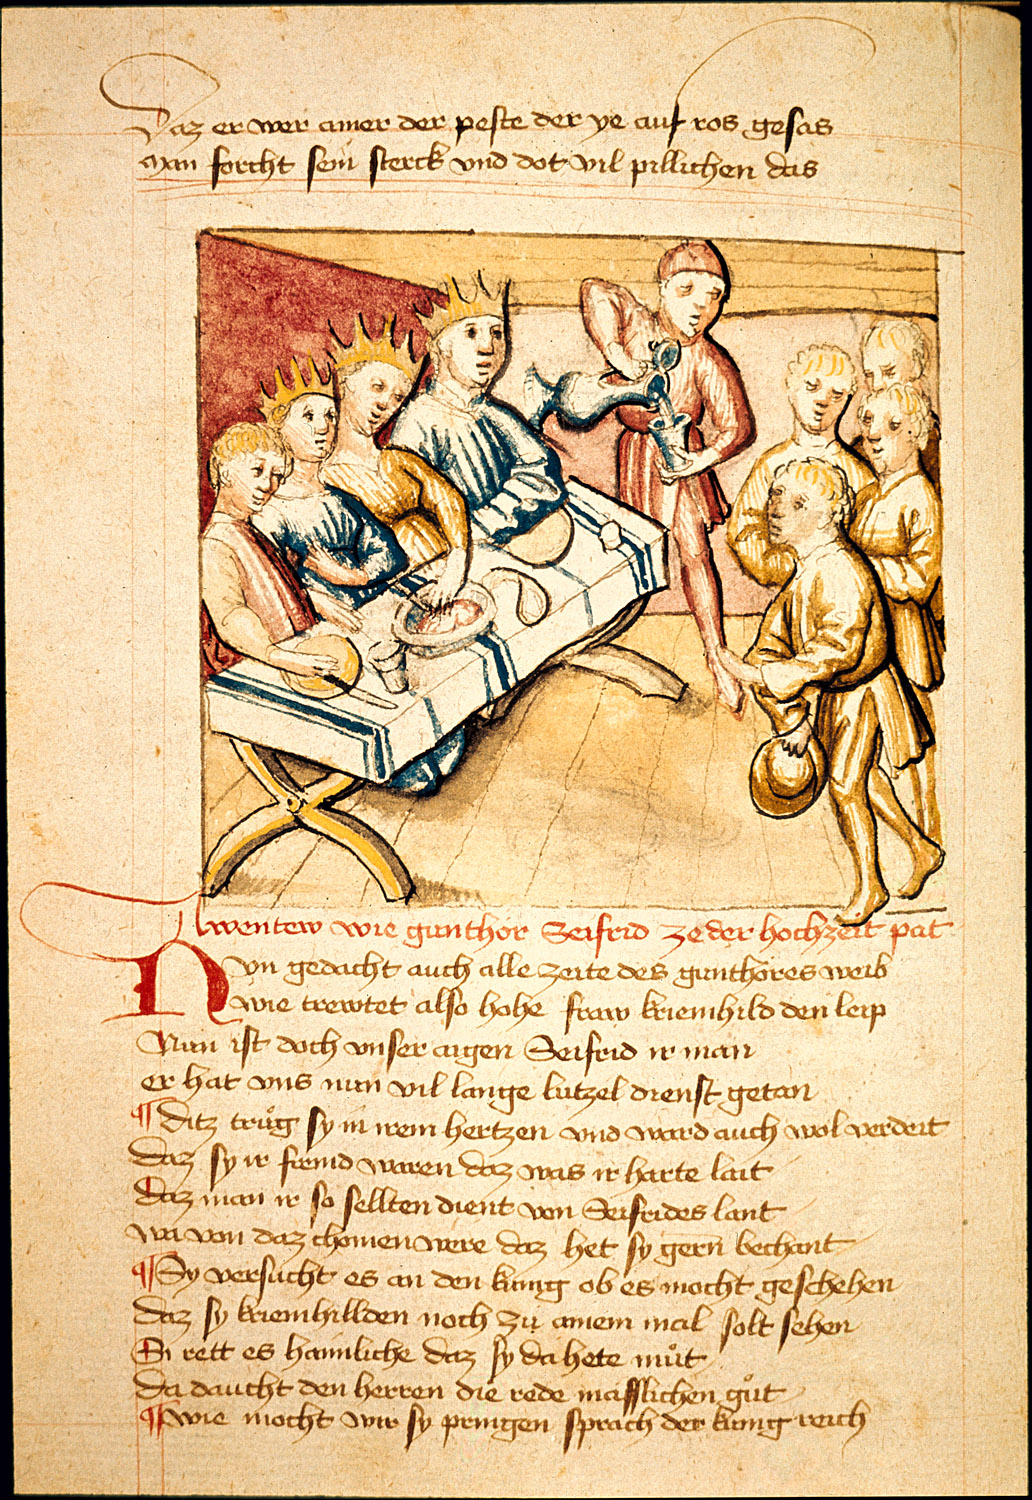
\includegraphics[width=3cm]{Scroll.jpg}
}
&~&
  \parbox{.3
\textwidth}{\tiny
  \Tree [.IP [ Roses ].NP_i [.I\1 [ are ].I\0
  [.VP t_i [ [ going ].V\0 \qroof{out of style}.PP ].V\1 ].VP
  ].I\1 ]
  } 
&~~~&
\parbox{.3\textwidth}{
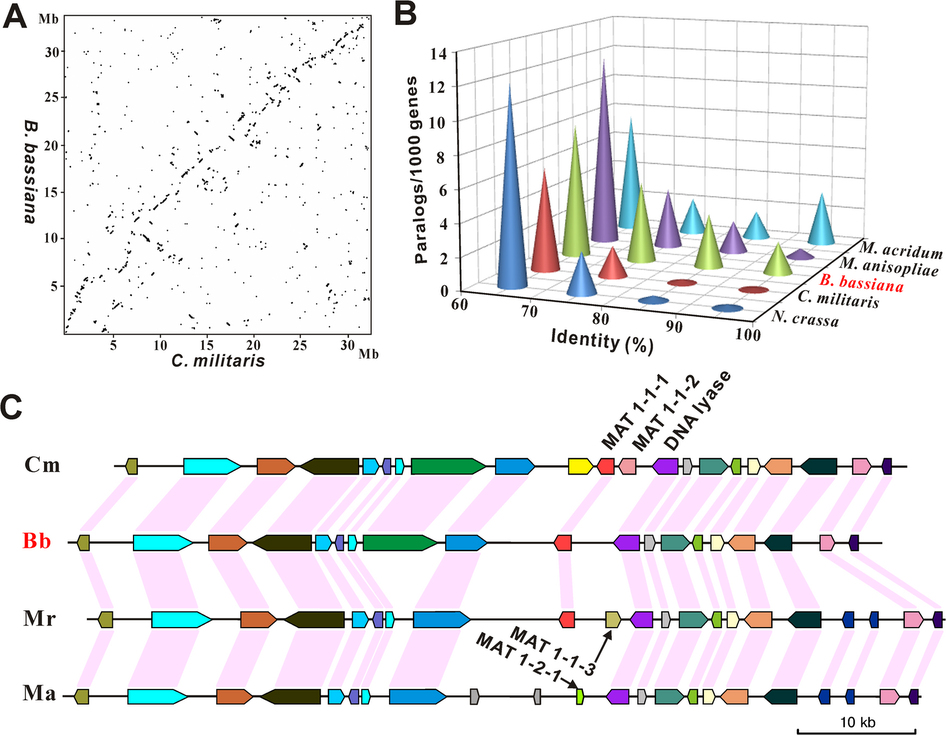
\includegraphics[width=3cm]{genome.jpg} 
\\
\begin{itemize}
 \item faster 
\item shorter
 \item more commodified
\end{itemize}

\vspace{1cm}
}
\end{tabular}
}

\frame{
\frametitle{Community}
 
\parbox{\textwidth}{
  \begin{tabular}{cc}
  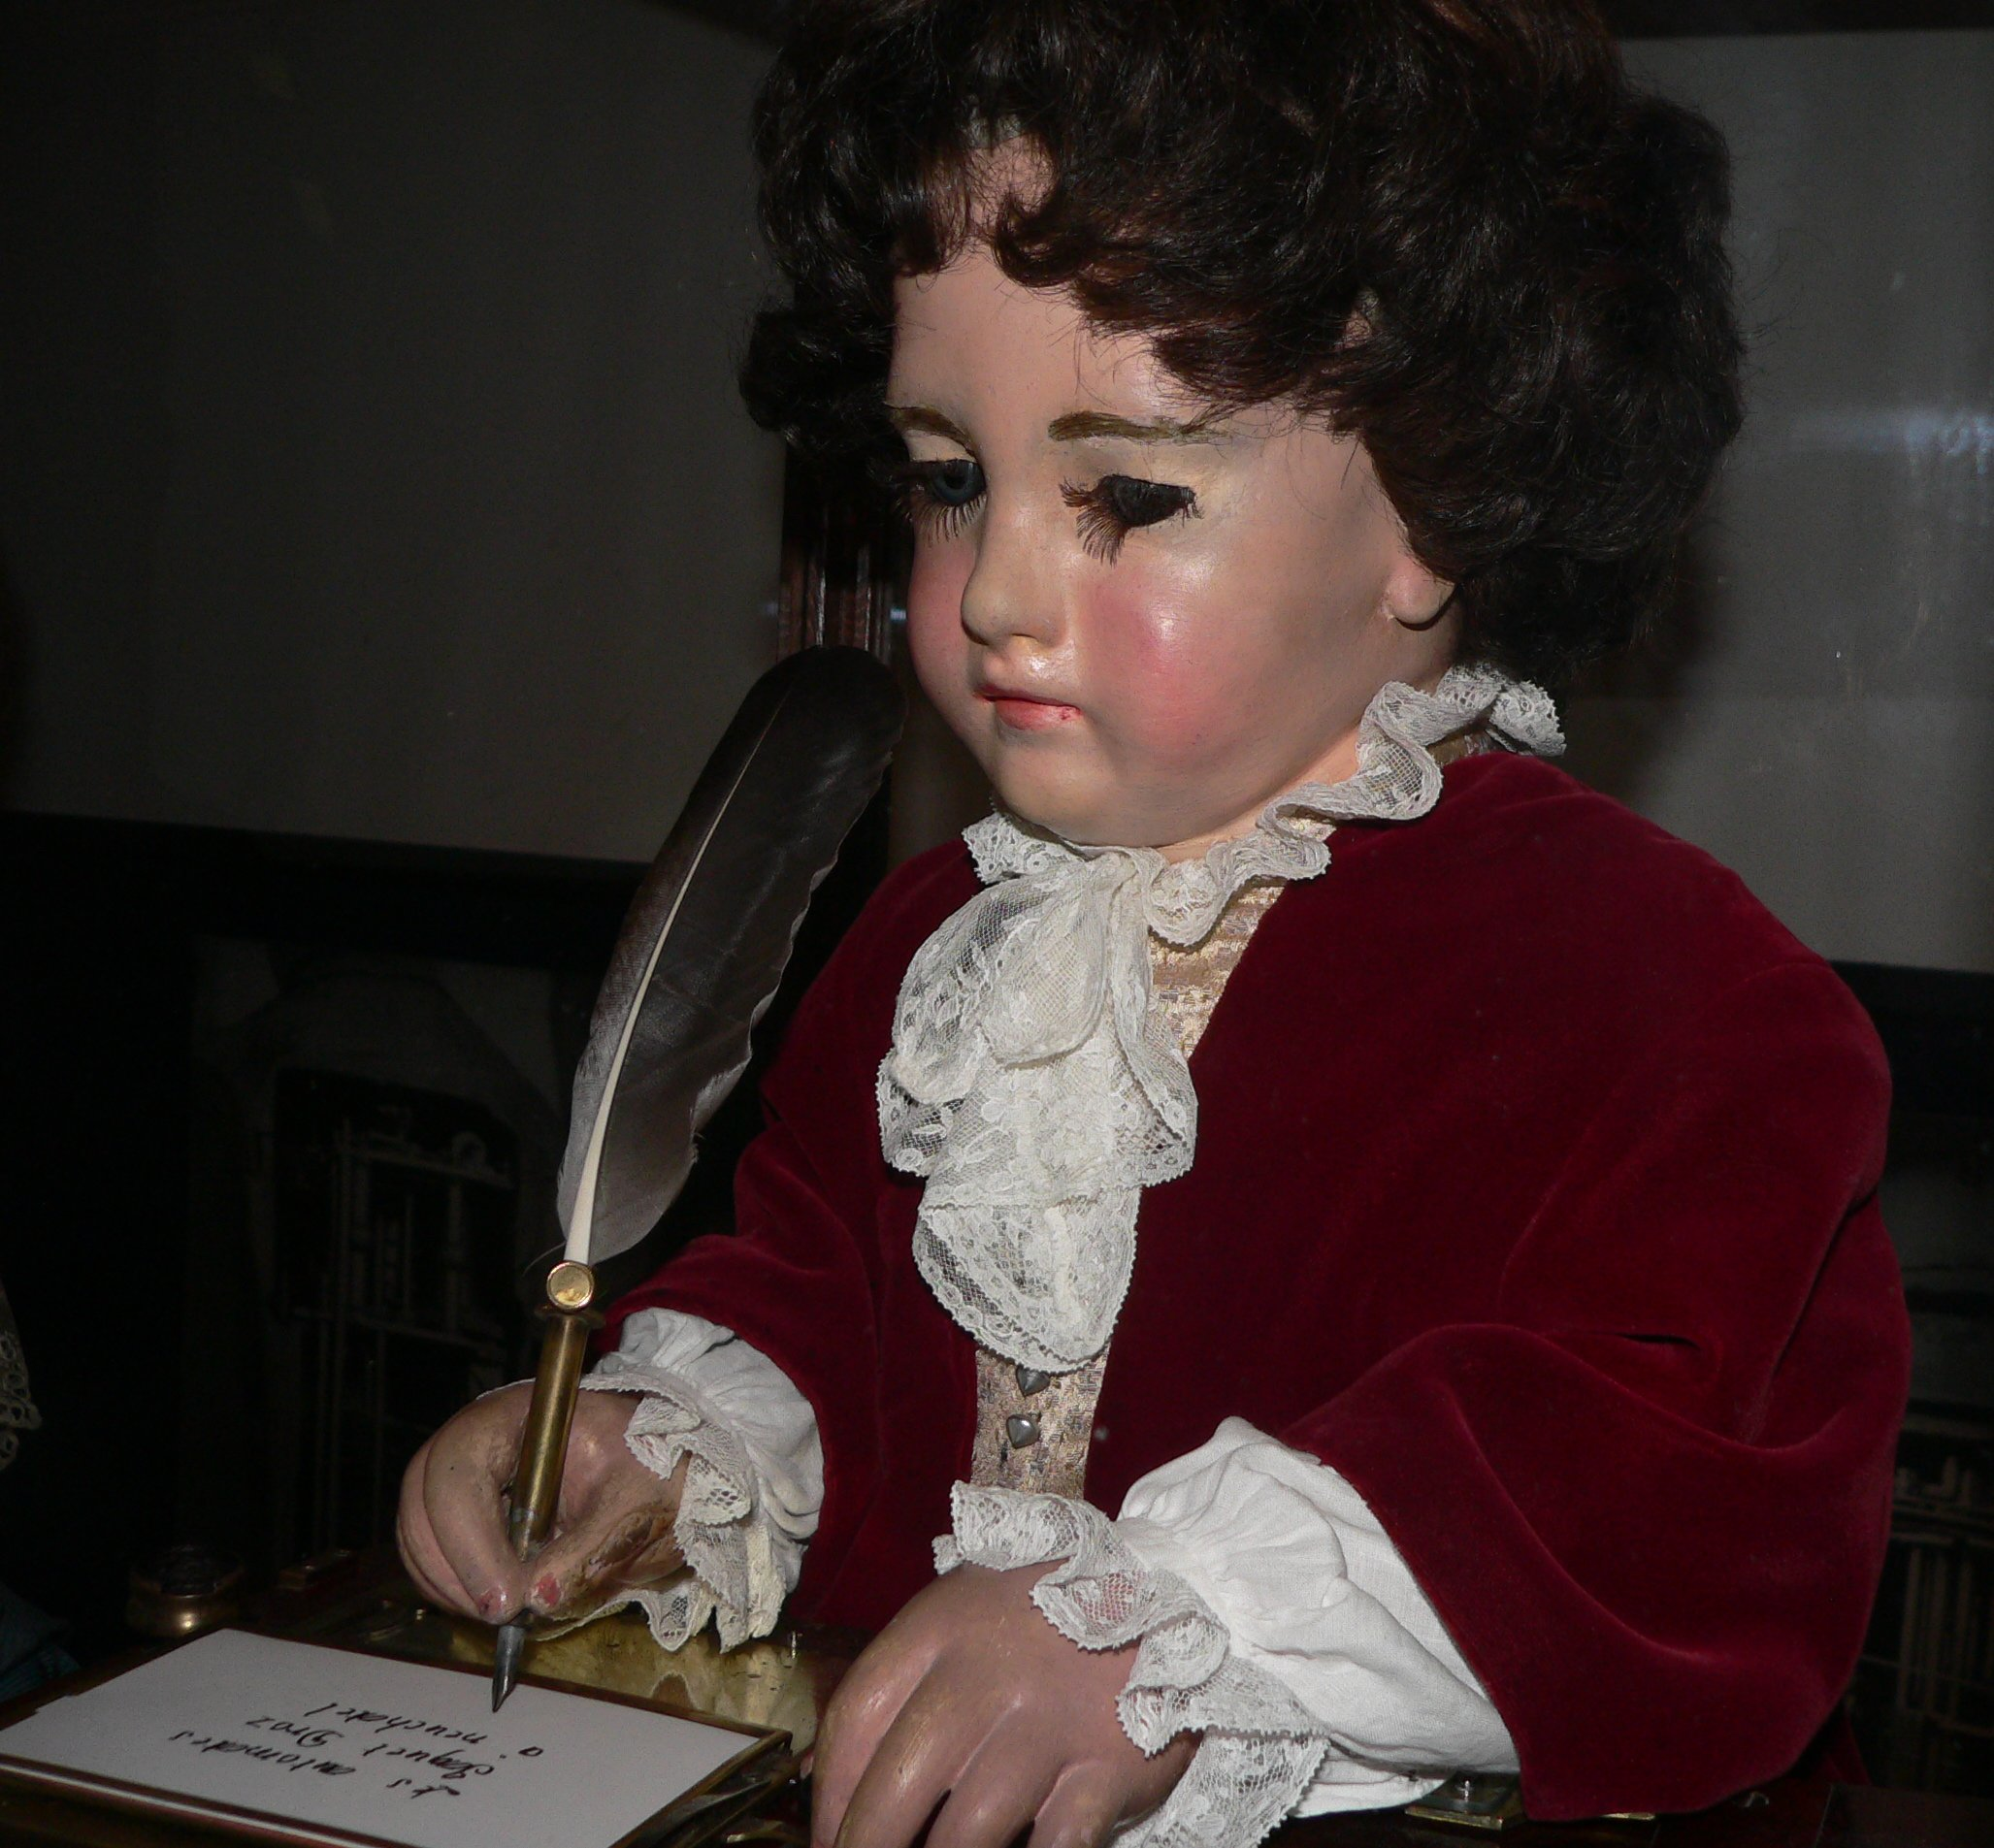
\includegraphics[width=.3\textwidth]{author.jpg}
  
  & ~~~~ ~~~~ ~~ ~
  
\includegraphics[width=.3\textwidth]{editor.png}
  \\ 
\hline
~~~~~ 
  
\includegraphics[width=.3\textwidth]{proofreader.png} 
&~~
  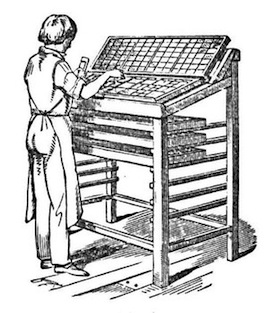
\includegraphics[width=.3\textwidth]{typesetter.jpg}   
  \end{tabular} 
} 



}

\frame{
\frametitle{World wide network}
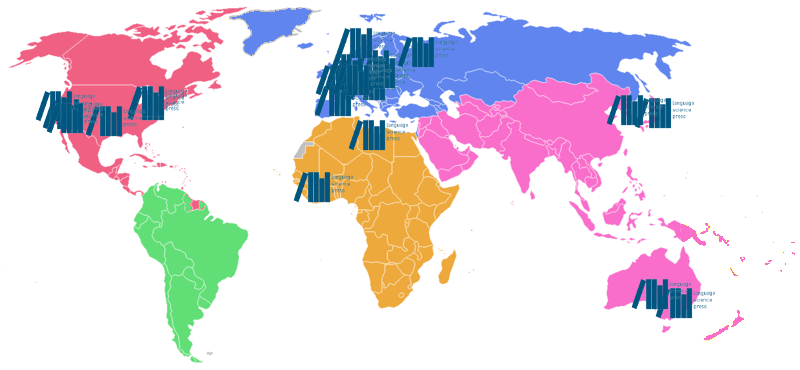
\includegraphics[width=1.2\textwidth]{worldmap.png} 
}

\frame{
\frametitle{Prestige}
\includegraphics[width=.6\textwidth]{bookpile.jpg}

\includegraphics[width=.3\textwidth]{oscar.jpg}
}



\frame{
\frametitle{Open Access, Open Source, Open Data}
\begin{tabular}{p{4.6cm}r}
% \parbox{.4\textwidth}{
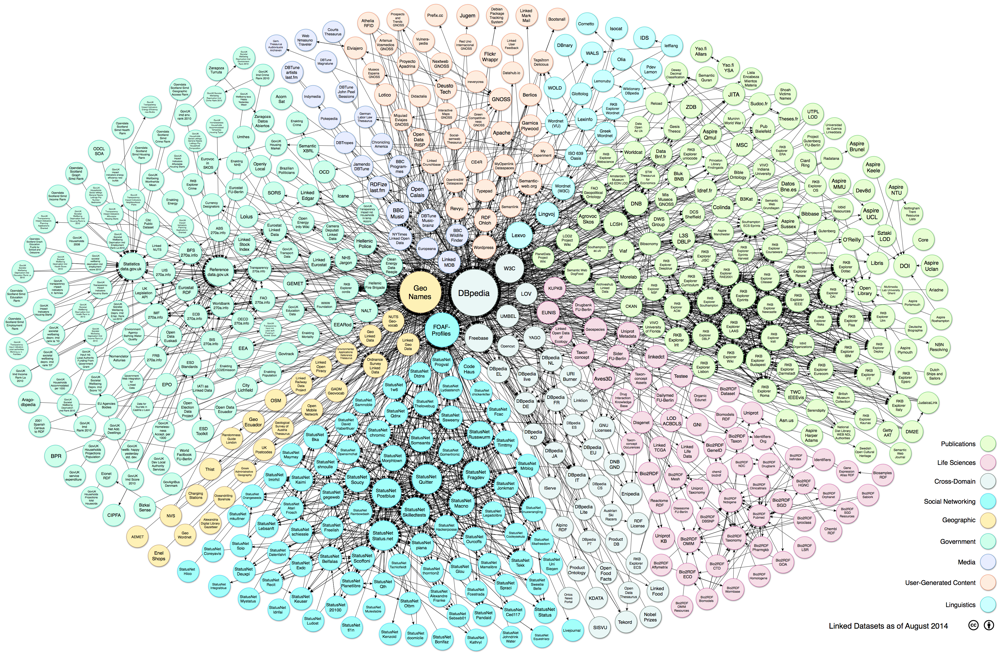
\includegraphics[height=1.1\textheight]{lod.png}
% }
& 
\parbox{.4\textwidth}{
\vspace{-4.4cm}
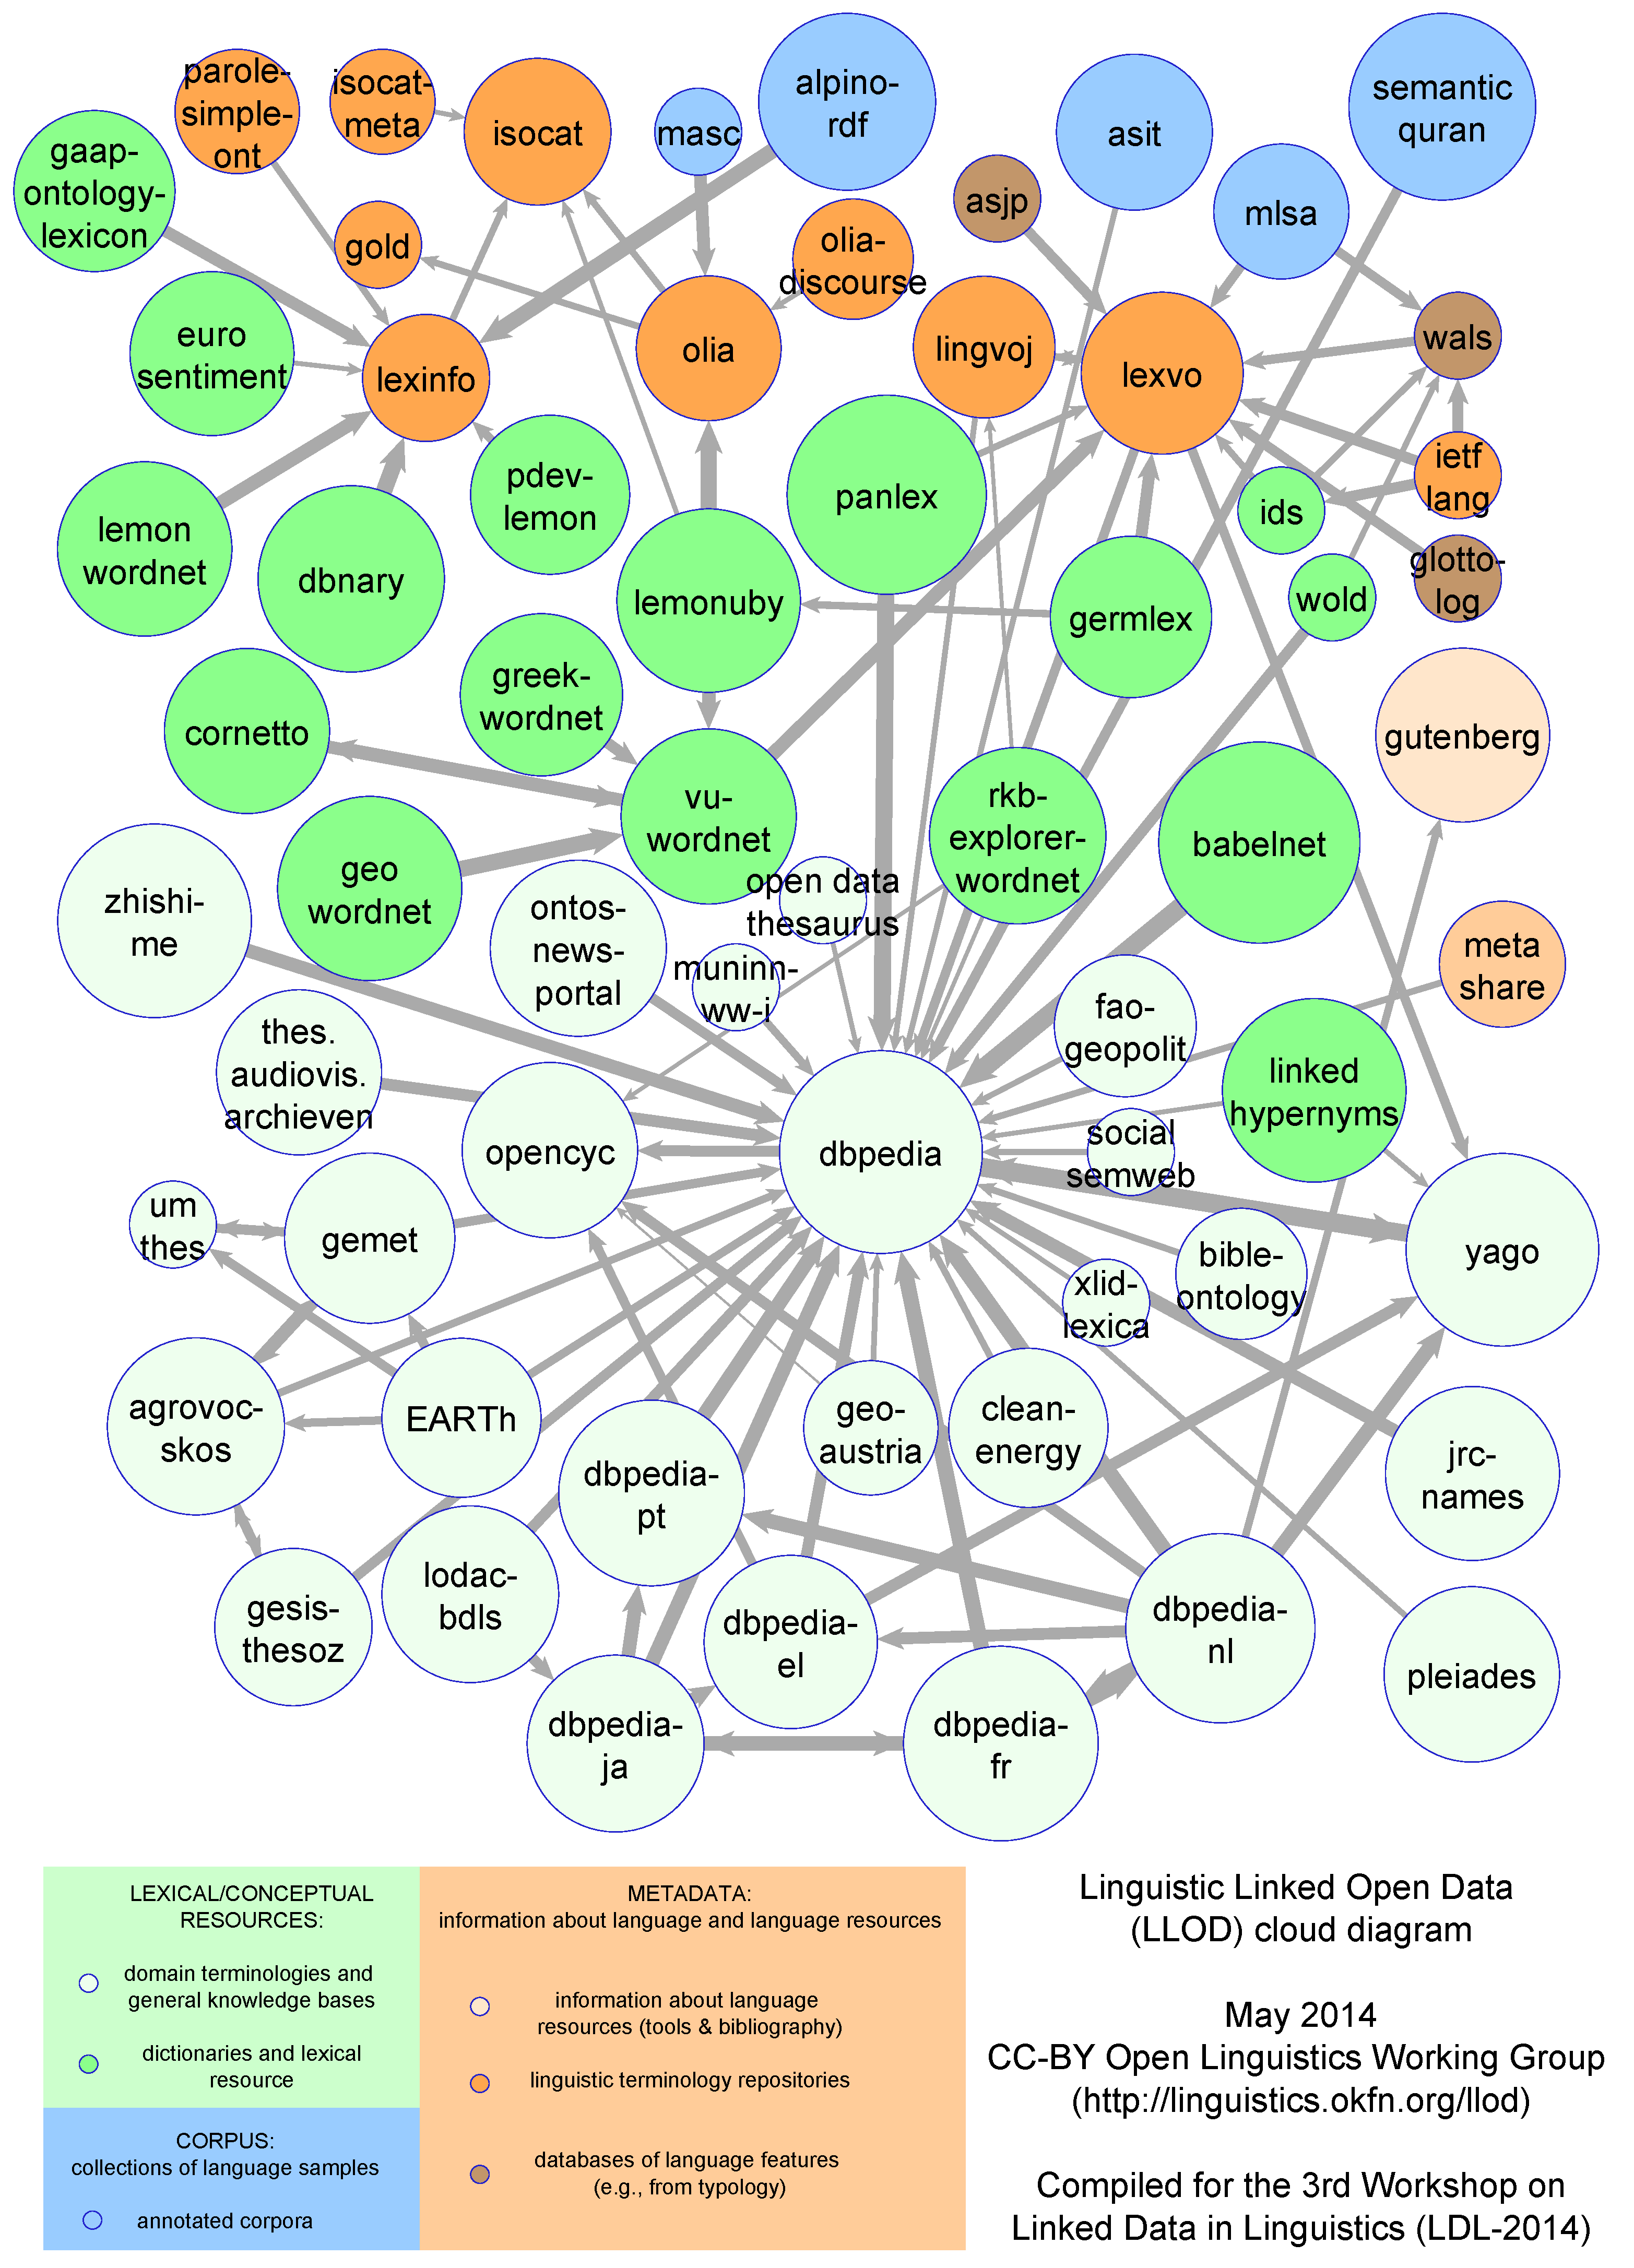
\includegraphics[height=1.5\textheight]{llod.pdf}
}
\end{tabular}

}
 

\setcounter{framenumber}{5}



\end{document}